\chapter{Previous Literature}
\label{cha:prev_literature}

The idea to reduce the amount of plastic wasted on supports with the use of better
generation algorithms is certainly not a new one, and there is a lot of ongoing
research on the topic. However most of the research is conducted by companies in 
the space, and by open source developers, with only a fraction of it ending up
in academic research. For this reason this section is divided into two parts,
in the first one we will give an overview of the papers that are adjacent
to this thesis (namely papers that apply genetic algorithms to ghe generation
of supports); In the second section we will take a look at the industry standard
algorithms for support generation.
The reason why this thesis considered solution coming from open source software, and 
from the industry, rather than limiting to the academic research that was available is simple:
The academic research on the topic is a quite sparse (only two papers were found at the time of writing).
Furthermore as we will discuss in section \ref{sec:limitations}, the approach taken by the authors is not
really suitable for FDM 3D printing, and focuses more on SLA. Moreover none of the related works in section \ref{sec:acc_lit}
have made the code available, and this make the process of comparison impossible.
For those reasons the choice was made to include in this section some solution taken from open source
software, as they are the defacto standard used for support generation by 3D printing enthusiast
allow us to properly evaluate the proposed algorithm with some simple comparison.

\section{Academic Literature}
\label{sec:acc_lit}

\subsection[Genetic-algorithm based framework for lattice support structure optimization]{Genetic-algorithm based framework for lattice support structure optimization in additive manufacturing \cite{VAISSIER201911}}
\label{sec:paper_1}

This paper was the first one to apply genetic algorithms to support structure generation, and did so with a relatively
straightforward approach. They began by identify the overhanging (i.e. the zones that required supports)
(figure \ref{fig:paper_1} part 1), then they used a procedural algorithm to design a grid around the structure
(figure \ref{fig:paper_1} part 2). In the next step (figure \ref{fig:paper_1} part 3) a pre-processing was applied to remove 
from the structures the beams that could be excluded from the solution ``A priori''. Step 4 followed, where 
a genetic algorithm was used to prune the structure and remove further unnecessary beams, in this step the cost
function applied was a simple function of the volume of the supports (figure \ref{fig:paper_1} part 4). Finally a simple 
post-processing algorithm was applied, in order to further reduce he material used (figure \ref{fig:paper_1} part 5).
This is done with a series of simple steps such as for example connecting every two beams series with an individual
beam that will always be the same length or shorter as the sum of the other two.


\begin{figure}[h]
    \centering
    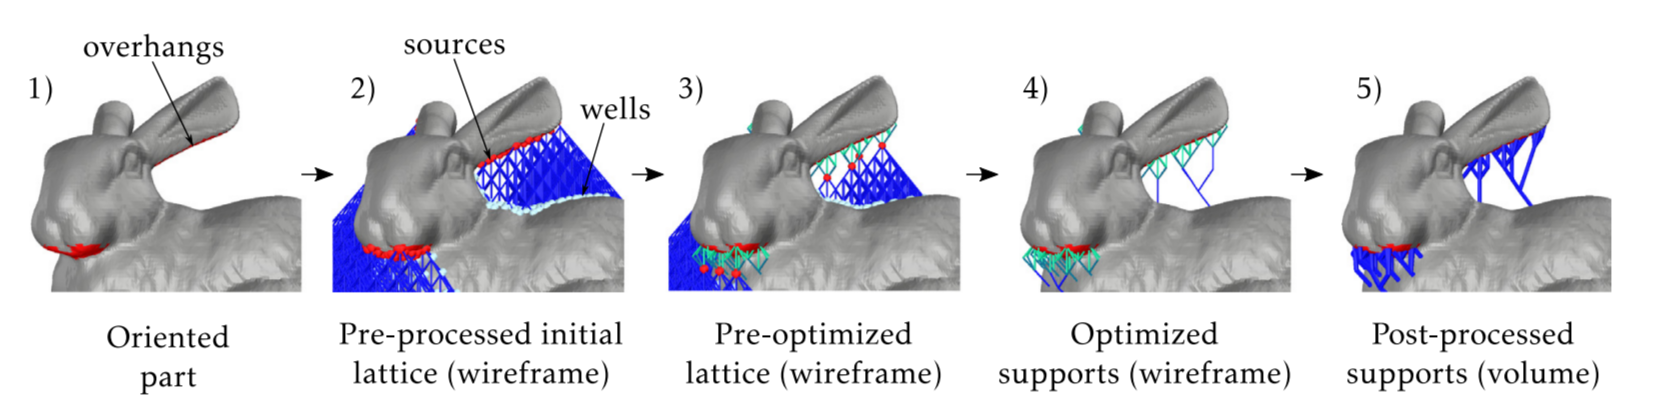
\includegraphics[width=0.95\textwidth]{images/paper1.png}
    \caption{Pipeline of paper \cite{VAISSIER201911}}
    \label{fig:paper_1}
\end{figure}

In the algorithm described above the grid was generated using a set of parameters (that were not subject to 
implicit optimization by the genetic algorithm) Those parameter were the height of a section, the distance
between the ``columns'', as well as the diameter of the beams, those parameters cam be seen in figure \ref{fig:paper_1_param}.
The authors emphasis how correctly selecting those parameters was essential for the quality of the results.


\begin{figure}[h]
    \centering
    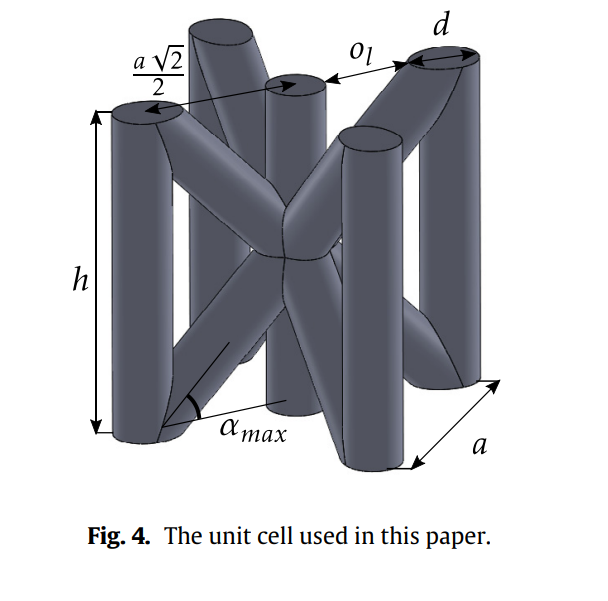
\includegraphics[width=0.4\textwidth]{images/paper1_params.png}
    \caption{Parameters used for structure (paper \cite{VAISSIER201911})}
    \label{fig:paper_1_param}
\end{figure}

The paper have also presented two different encoding structures to use in the optimization part (shown in figure \ref{fig:paper_1_encoding}).
The first strategy was called ``Activation Encoding'' where every beam of the graph was assigned
a boolean variable, where 0 meant that the node was removed, and 1 meant that the node was kept.
The first strategy was called ``Switch Node Encoding'' and essentially assumed every node could only be connected
to one of the possible downward directions, and the encoded variable simply selected one of the possible one.
The authors have shown how this approach drastically reduced the size of the search space, and made the optimizer's 
life a lot easier, thus making it faster and more accurate.


\begin{figure}[h]
    \centering
    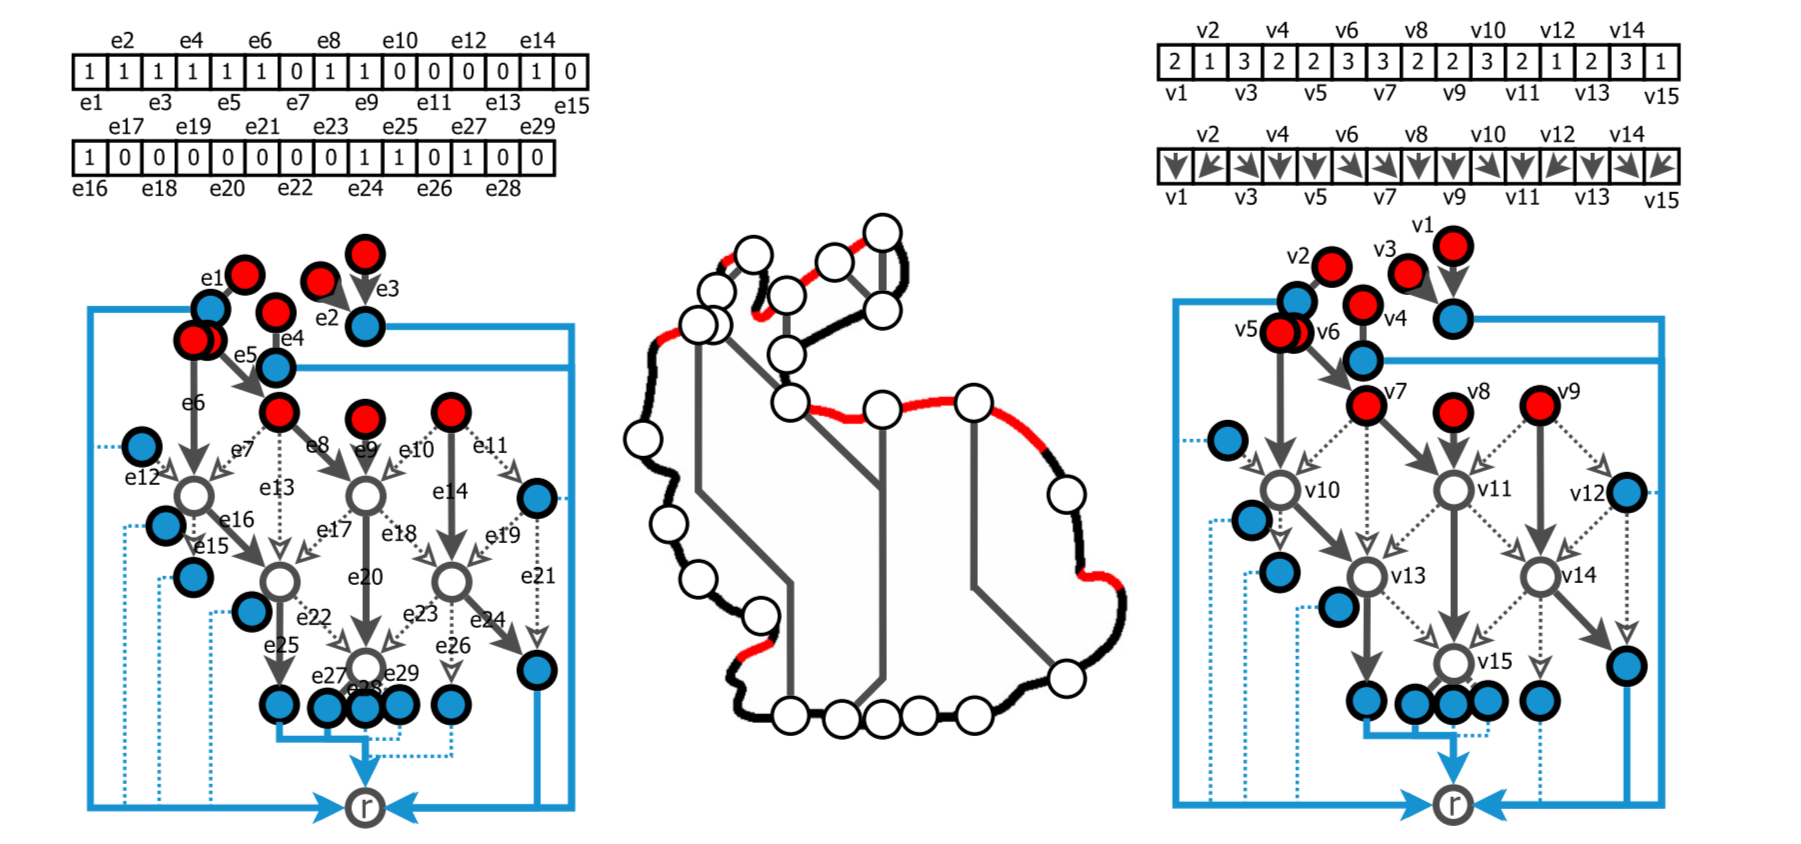
\includegraphics[width=0.95\textwidth]{images/paper1_encoding.png}
    \caption{The activation encoding (left), and switch node encoding (right) (paper \cite{VAISSIER201911})}
    \label{fig:paper_1_encoding}
\end{figure}

The paper concluded by testing the algorithm in a variety of meshes, and against a variety of support generation
algorithms selected from a academic papers, and a variety of industry standard tools.
They shown how their framework managed to reduce the use of material by 10-20\% compared to the the previous
best results.
The paper also shown one real world print made with their algorithm using a Laser Beam Melting (LBM) 3D printer
(which is a technology conceptually pretty similar to SLS). In conclusion this paper is quite relevant to the
work conducted in this thesis, as it's the first application of genetic algorithms for support structure optimization.
However their work was heavily focuses on LBM, and due to a set of factor that we will explain
in section \ref{sec:limitations} is not really applicable to FDM 3D printing.



\subsection[Bio-inspired generative design for support structure generation and optimization in Additive Manufacturing (AM)]{Bio-inspired generative design for support structure generation and optimization in Additive Manufacturing (AM) \cite{ZHANG2020117}}
\label{sec:paper_2}

This paper was also an developed with the idea to apply genetic algorithms to the problem of supports structure
optimization. The key novelty here was the introduction of a multi objective optimization program.
While in the previous paper \ref{sec:paper_1} the objective function was limited to minimizing the volume, in this
paper they focus on minimizing both the volume and the collisions \ref{fig:paper_2_collisions} among the support and the printed object.
Minimizing collisions is essential to ensure that the supports are easy to remove.
In order to optimize not only a single solution, but the set of pareto-optimal solution the authors used
the NSGA-II algorithms.

\begin{figure}[h]
    \centering
    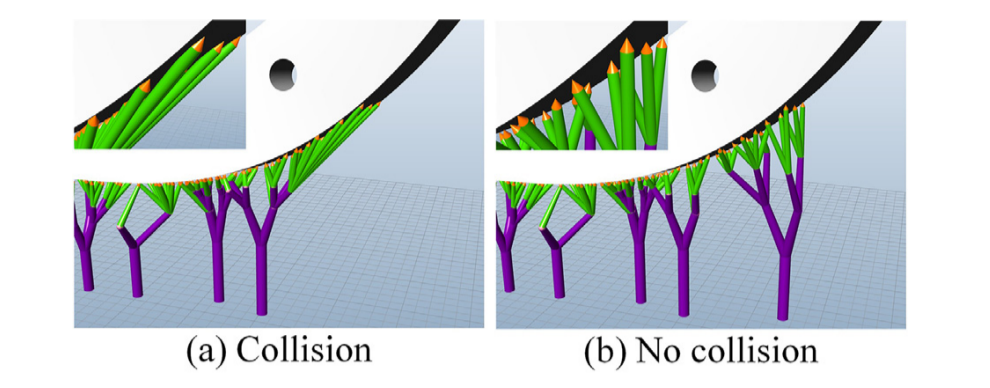
\includegraphics[width=0.5\textwidth]{images/paper_2_collisions.png}
    \caption{Collisions between the supports and the model (paper \cite{ZHANG2020117})}
    \label{fig:paper_2_collisions}
\end{figure}

One key novelty of this paper is the use of a dual stage optimization approach. They infact decided to
split the optimization into two separate problems. In the first one they find the critical structures, and they then
proceed to optimize the set of ``contact points'' (i.e. the position where the support structure will attach to the object)
This optimization problem is solved, and then they move on to the second stage, in which they used an L-System \ref{fig:paper_2_l_system}
who's parameters where optimized by genetic algorithms to optimize the structure of the trees.


\begin{figure}[h]
    \centering
    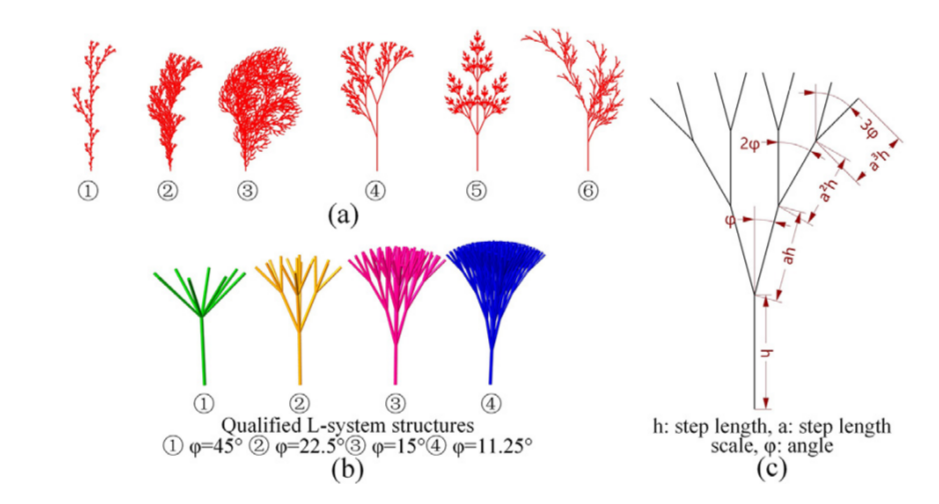
\includegraphics[width=0.5\textwidth]{images/paper_2_l_system.png}
    \caption{L-system used by zhang et. al. 2020 \cite{ZHANG2020117}}
    \label{fig:paper_2_l_system}
\end{figure}

Finally after a post-processing step that select one solution out of the evolved solution
a support structure is obtained. In the paper they tested the algorithm against
a collection of similar software and found that the reduction in use of material was approximately
40\%, Although it is wrath noting that they did only test prints of one object.
Nevertheless, the results are quite good, and can be seen in figure \ref{fig:paper_2_results}

\begin{figure}[h]
    \centering
    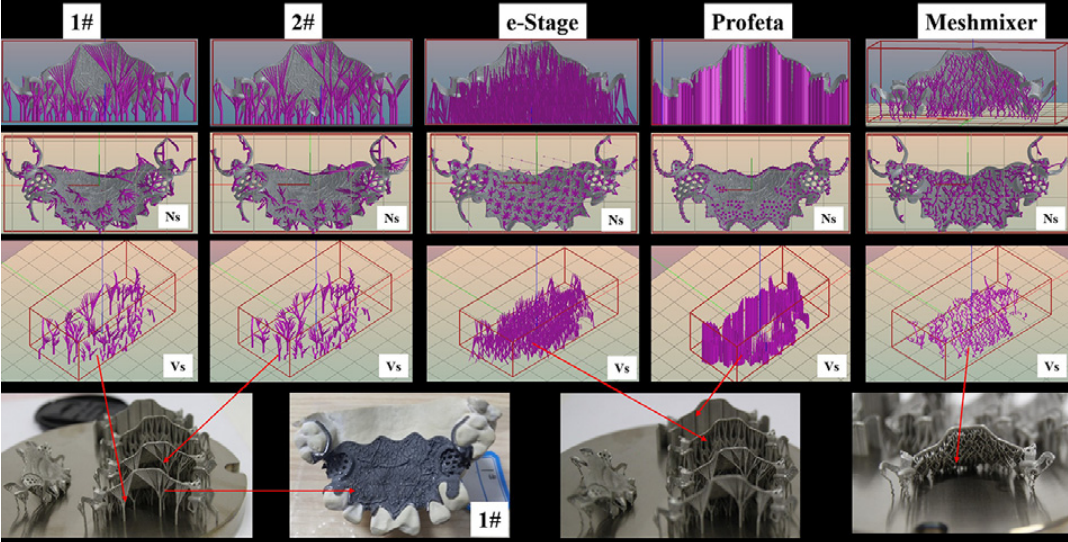
\includegraphics[width=0.5\textwidth]{images/paper_2_results.png}
    \caption{Result of zhang et. al. 2020 \cite{ZHANG2020117}}
    \label{fig:paper_2_results}
\end{figure}


\section{Industry Standard Solutions}


The Academic literature that was reviewed in the previous section is primarily geared towards
an industrial settings, and is therefore more focused on SLS  technologies (or similar), however
this thesis is more centered around the FDM technologies, and is therefore trying to solve a set 
of problems that is slightly different with respect to the papers that we just reviewed.
For this reason a second class of ``state of the art'' solutions is presented here.
This is a collection of support generation algorithms taken from the most used slicer for FDM printers
on the market.
The primary option to choose from here were OrcaSlicer \cite{orca_slicer} and Cura \cite{cura}.
However after a quick test it become clear that OrcaSlicer's support algorithms are superior
to cura in terms of material use, therefore they were selected as the key benchmark.

\subsection{``Normal Support'' (Orca slicer)}
\label{sec:normal_supports}

Normal supports are the one of the first example of auto-generated supports for 3D printing,
they are nothing special, as they are limited to a uniform wall create a zig-zag pattern in order
to reach the criticality region.
Compared to other techniques such as Tree support \ref{sec:tree_support}, those are considered a bit
wasteful.
Their inefficiency is simply given by the fact that the design is a straight wall that connect the critical
section at the top to the building plate as the bottom. Other more optimized algorithms try to merge multiple
critical areas together, in order to generate a single support that is narrower at the bottom, and brach out at the
top. This of course reduces the required materials.
Another key feature of modern support generation algorithms, that this algorithm doesn't have is a clean way
to handle supports that are ``multi layer'' (defined as a critical area that instead of having a direct line of sight
to the build plate have another part of the printed object that block the direct path from the critical area to the floor).
e can see this clearly in figure \ref{fig:multi-layer-support},
where the the normal support algorithm, when faced with a ``multi layer'' support, simply create a structure that go
straight down, and that rest on the printed object. This is generally considered undesirable, as it create twice
as many contact point between the support and the object, thus making the support removal  process more complicated.


\begin{figure}[h]
    \centering
    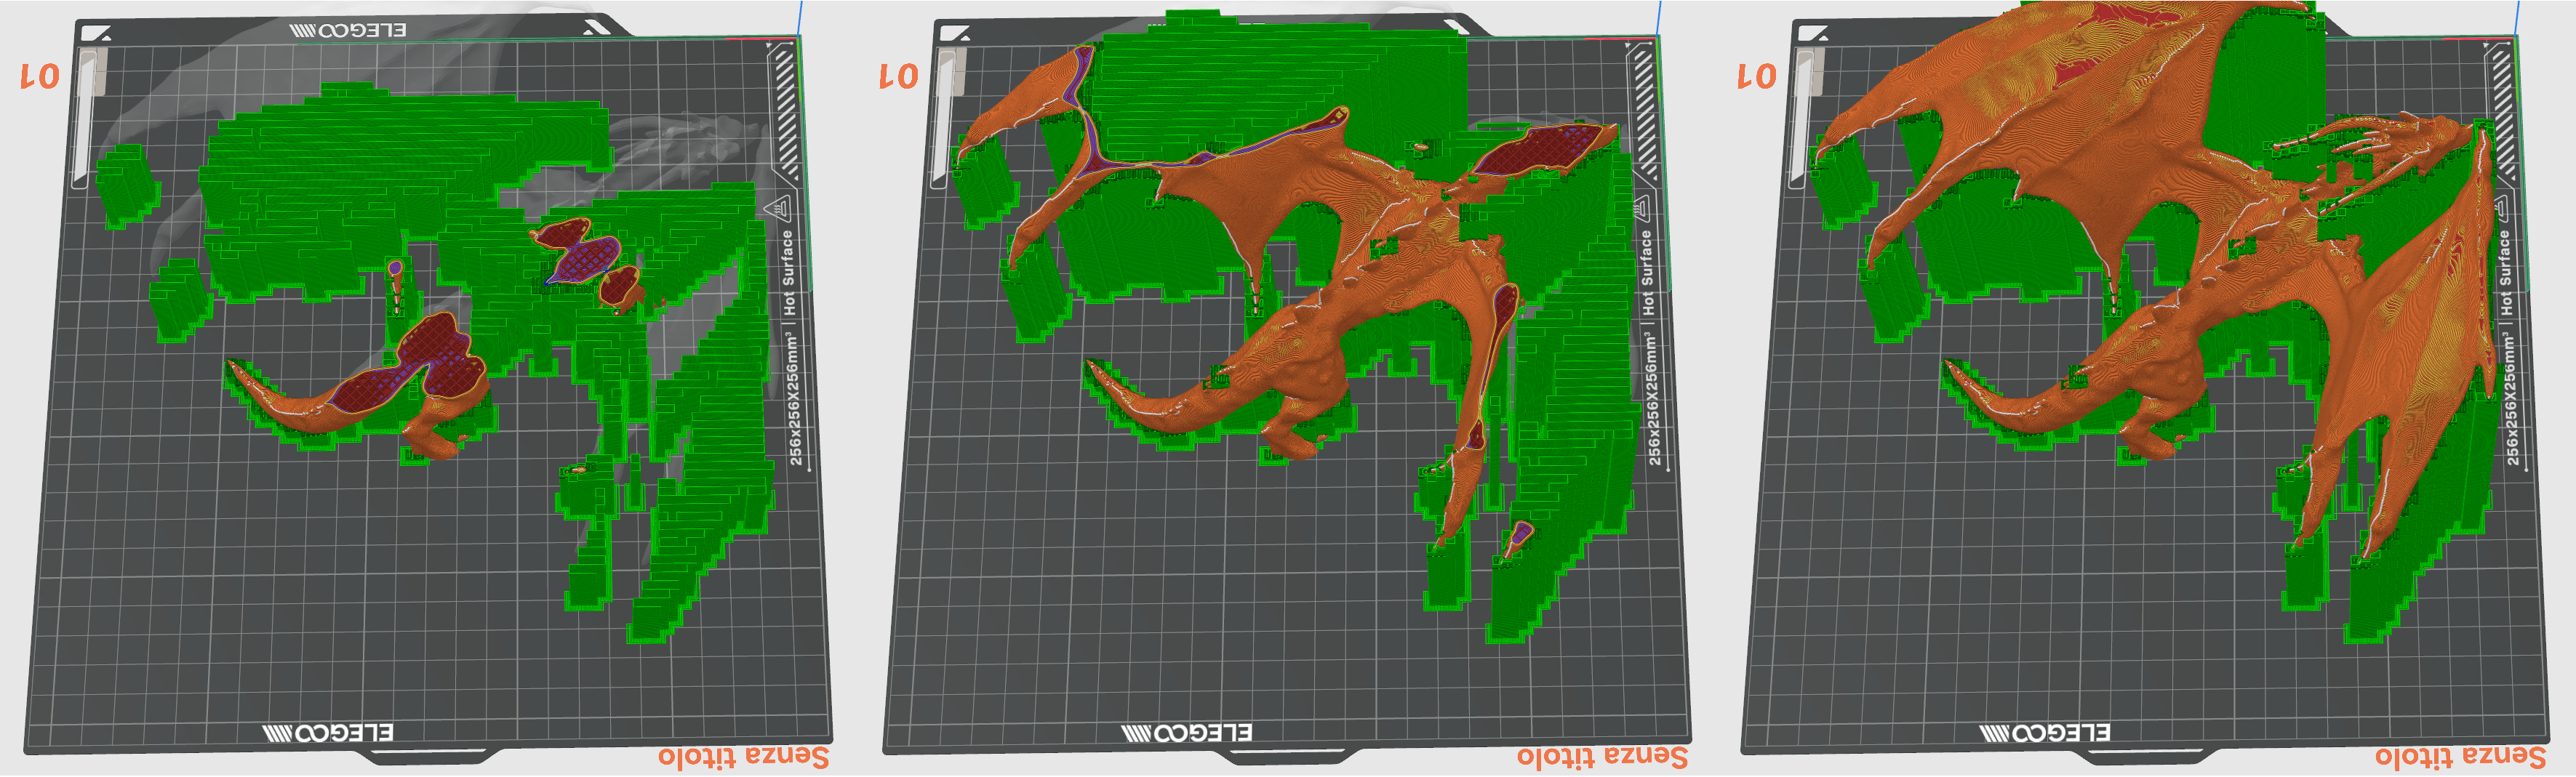
\includegraphics[width=1.0\textwidth]{images/normal_support.png}
    \caption{Normal supports (orca slicer)}
    \label{fig:normal_supports}
\end{figure}




\subsection{``Tree Supports'' (Orca slicer)}
\label{sec:tree_support}

Tree supports are the modern gold standard for lean support structure of FDM 3D printing.
They are a relatively new idea with the first version of their current form tracing back to 
an alpha release of Cura in late 2022 \cite{tree_supports}.
Every since then they have only improved, and they have become a beloved by the community.
Their design is incredibly simple and yet effective, critical regions that are close together
are merged into a single brach that move towards the plate, and gradually merge with other branches.
This is ensuring that the taller a critical area is, the more likely it is that it's support
will merge with others while moving towards the blate. This has proven very effective in reducing
the amount of material, as every two branches are merged we remove the need of having two
independent structures that go up to a certain height.

One key feature of tree support that should not be overlooked is the fact that the tree structures
are thicker at the bottom and they gradually get skinnier at the top. This is essential to ensure that
the supports can be printed correctly, as having supports that are too skinny at the bottom
would cause a z-wobble effect \ref{fig:wobble-test}, and thus leading to a failure.
It is also important to note that the tree get skinnier as it grows in order to save material, this can be done
due to the fact that when the nozzle is applying force by depositing the filament, the tree itself
is acting as a lever (with the fulcrum being the plate, and the force being applied where the nozzle is), 
and therefore the closer you are to are to the nozzle, the less advantageous the lever become, thus reducing
the amount of stiffness that the tree need to provide in order to not bend.



\begin{figure}[h]
    \centering
    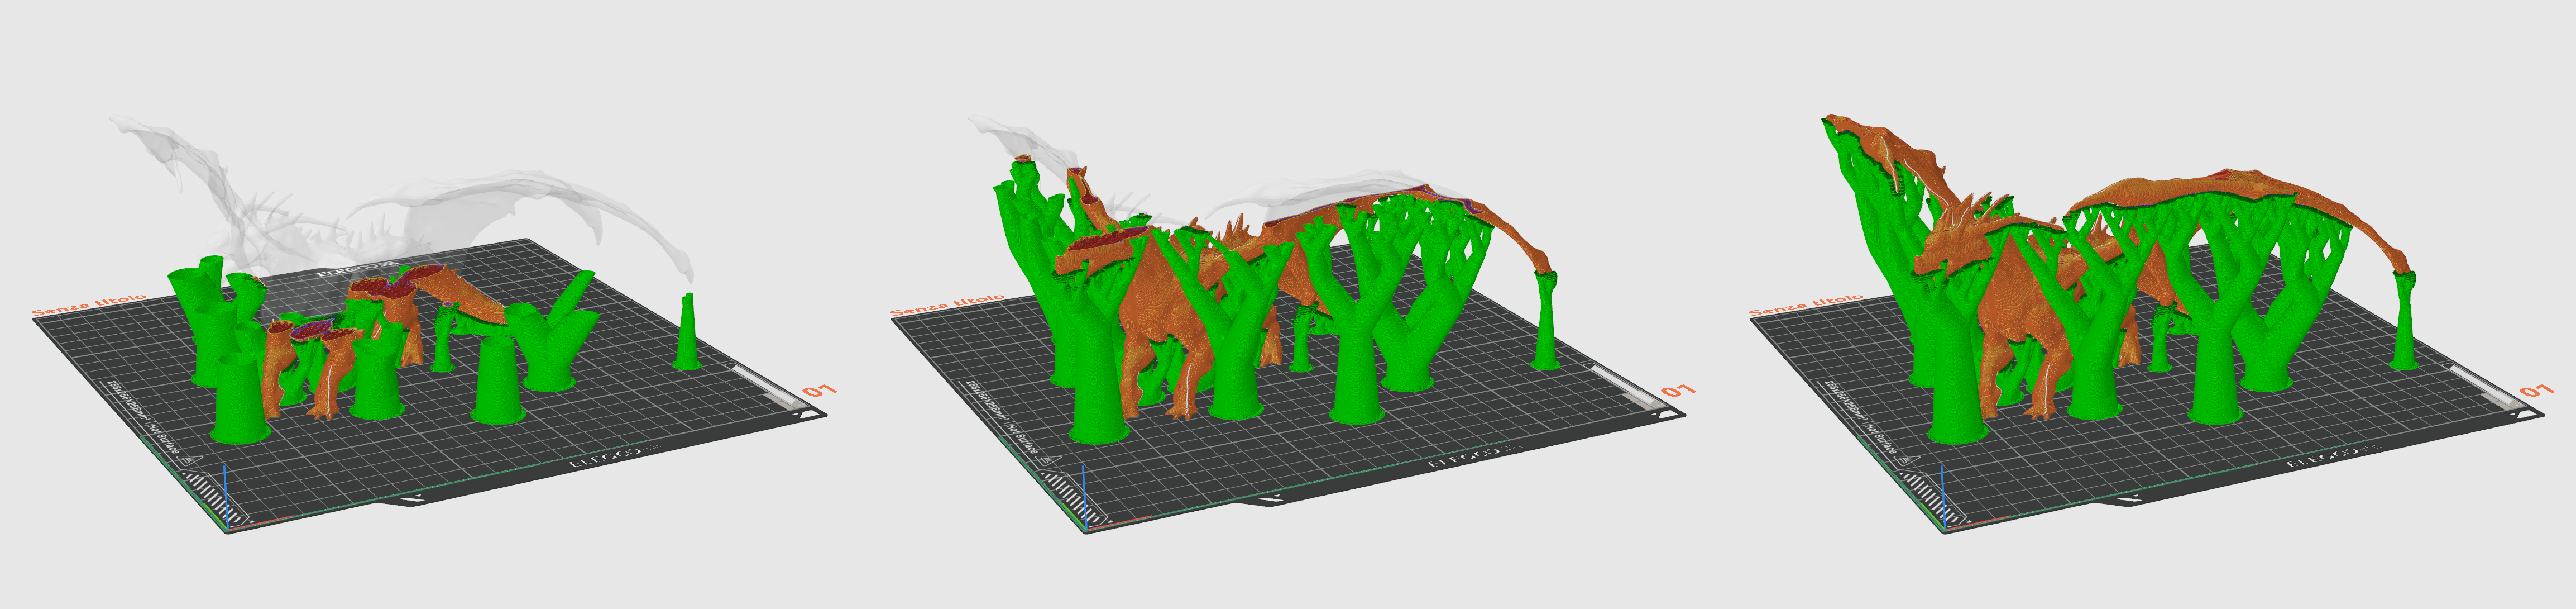
\includegraphics[width=1.0\textwidth]{images/tree_support.png}
    \caption{Tree supports (orca slicer)}
    \label{fig:tree_supports}
\end{figure}

One final feature of the tree supports is the way they handle ``multi layer supports'' (defined in \ref{sec:normal_supports})
As you can see in figure \ref{fig:multi-layer-support} when faced with this circumstance the algorithm try to find a diagonal
route that manage to support the critical area without intersecting with the printed object. This is feature is quite
liked by the community as it makes the supports easier to detach, even tho it increases slightly the amount of materials required 
for the supports.

\begin{figure}[h]
    \centering

    \begin{minipage}{0.48\textwidth}
        \centering
        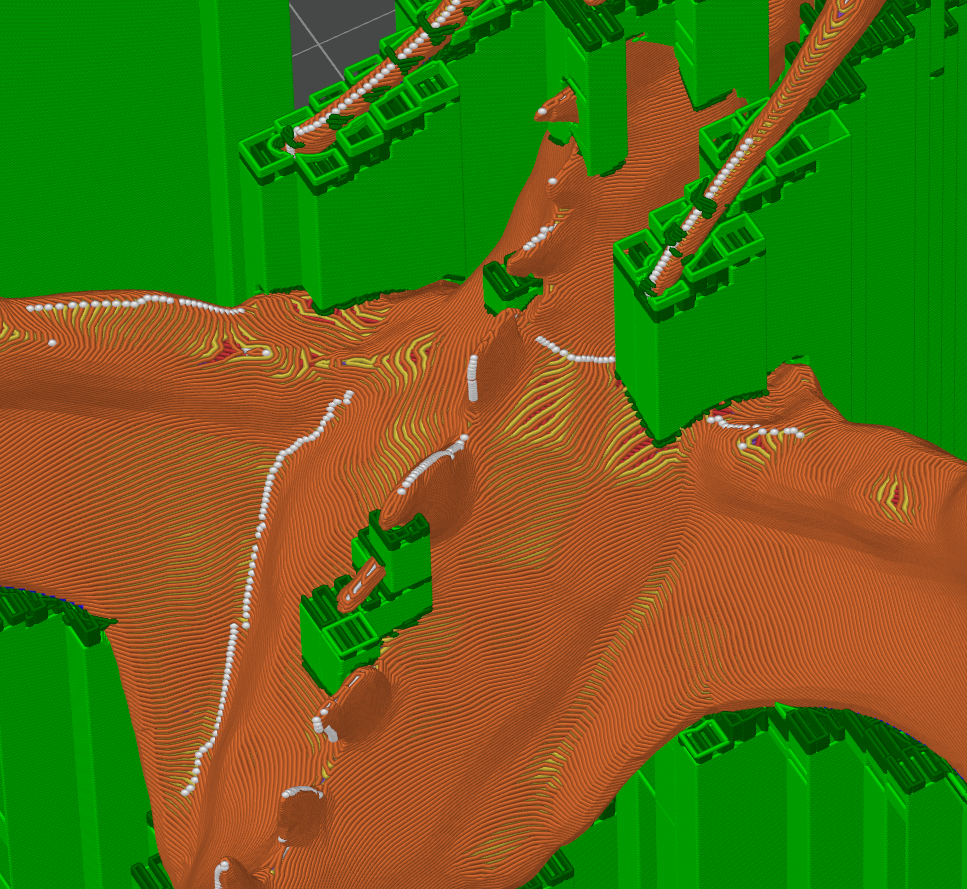
\includegraphics[width=0.9\textwidth]{images/munti_layer_supports_normal.png}
    \end{minipage}
    \hfill
    \begin{minipage}{0.48\textwidth}
        \centering
        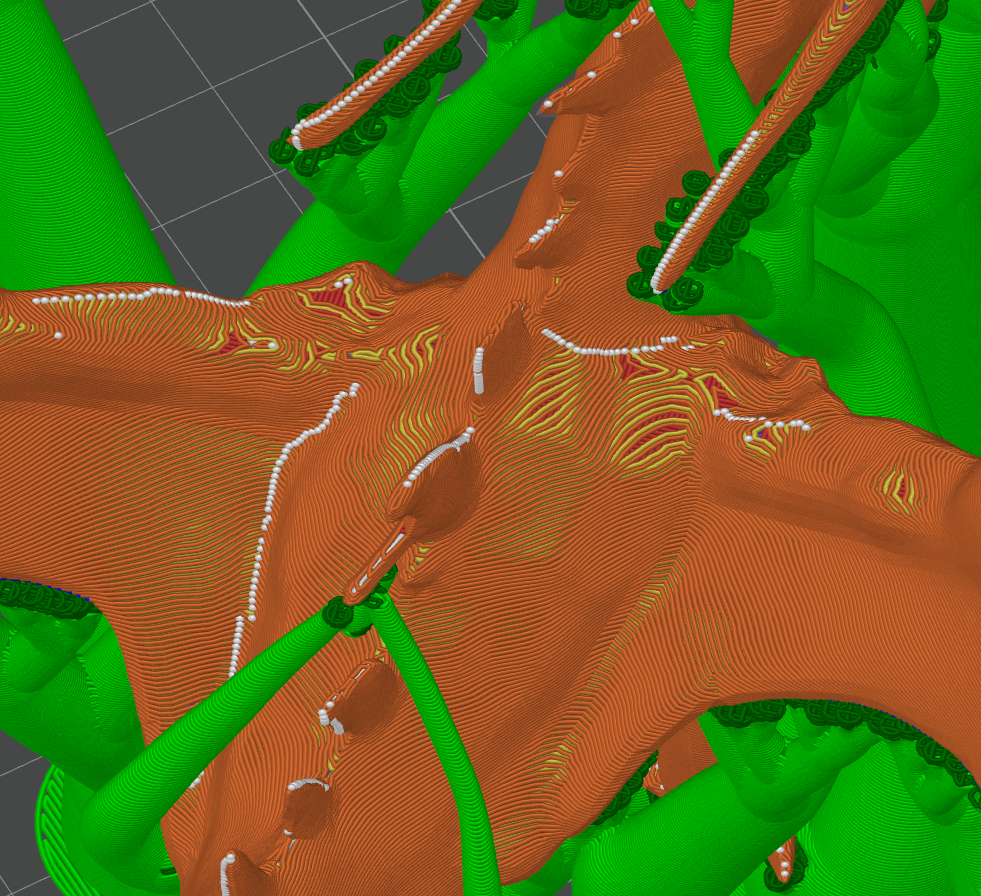
\includegraphics[width=0.9\textwidth]{images/multi_layer_supports_tree.png}
    \end{minipage}

    \caption{Handle of multi-layer supports (left: Normal supports, right: Tree supports)}
    \label{fig:multi-layer-support}
\end{figure}







